\documentclass[
11pt, % The default document font size, options: 10pt, 11pt, 12pt
%codirector, % Uncomment to add a codirector to the title page
]{charter} 




% El títulos de la memoria, se usa en la carátula y se puede usar el cualquier lugar del documento con el comando \ttitle
\titulo{Uso de técnicas de visión por computadora para mejorar la precisión de un sistema autónomo de checkout} 

% Nombre del posgrado, se usa en la carátula y se puede usar el cualquier lugar del documento con el comando \degreename
%\posgrado{Carrera de Especialización en Sistemas Embebidos} 
%\posgrado{Carrera de Especialización en Internet de las Cosas} 
\posgrado{Carrera de Especialización en Inteligencia Artificial}
%\posgrado{Maestría en Sistemas Embebidos} 
%\posgrado{Maestría en Internet de las cosas}

% Tu nombre, se puede usar el cualquier lugar del documento con el comando \authorname
\autor{Ing. Rodrigo Pazos} 

% El nombre del director y co-director, se puede usar el cualquier lugar del documento con el comando \supname y \cosupname y \pertesupname y \pertecosupname
\director{Ing. Maxim Dorogov}
\pertenenciaDirector{FIUBA} 
% FIXME:NO IMPLEMENTADO EL CODIRECTOR ni su pertenencia
\codirector{John Doe} % para que aparezca en la portada se debe descomentar la opción codirector en el documentclass
\pertenenciaCoDirector{FIUBA}

% Nombre del cliente, quien va a aprobar los resultados del proyecto, se puede usar con el comando \clientename y \empclientename
\cliente{Direccion de la carrera de CEIA}
\empresaCliente{FIUBA}

% Nombre y pertenencia de los jurados, se pueden usar el cualquier lugar del documento con el comando \jurunoname, \jurdosname y \jurtresname y \perteunoname, \pertedosname y \pertetresname.
\juradoUno{Nombre y Apellido (1)}
\pertenenciaJurUno{pertenencia (1)} 
\juradoDos{Nombre y Apellido (2)}
\pertenenciaJurDos{pertenencia (2)}
\juradoTres{Nombre y Apellido (3)}
\pertenenciaJurTres{pertenencia (3)}
 
\fechaINICIO{20 de junio de 2023}		%Fecha de inicio de la cursada de GdP \fechaInicioName
\fechaFINALPlan{15 de agosto de 2023} 	%Fecha de final de cursada de GdP
\fechaFINALTrabajo{abril de 2024}	%Fecha de defensa pública del trabajo final


\begin{document}

\maketitle
\thispagestyle{empty}
\pagebreak


\thispagestyle{empty}
{\setlength{\parskip}{0pt}
\tableofcontents{}
}
\pagebreak


\section*{Registros de cambios}
\label{sec:registro}


\begin{table}[ht]
\label{tab:registro}
\centering
\begin{tabularx}{\linewidth}{@{}|c|X|c|@{}}
\hline
\rowcolor[HTML]{C0C0C0} 
Revisión & \multicolumn{1}{c|}{\cellcolor[HTML]{C0C0C0}Detalles de los cambios realizados} & Fecha      \\ \hline
0      & Creación del documento.                                 &\fechaInicioName \\ \hline
1      & Se completa hasta el punto 5 inclusive.                 & 4 de julio de 2023 \\ \hline
2      & Se completa hasta el punto 9 inclusive.                & 11 de julio de 2023 \\ \hline
3      & Se completa hasta el punto 12 inclusive.                & 25 de julio de 2023 \\ \hline
4      & Se completa hasta el punto 15 inclusive.                & 1 de agosto de 2023 \\ \hline
%2      & Se completa hasta el punto 7 inclusive
%		  Se puede agregar algo más \newline
%		  En distintas líneas \newline
%		  Así                                                    & dd/mm/aaaa \\ \hline
%3      & Se completa hasta el punto 11 inclusive                & dd/mm/aaaa \\ \hline
%4      & Se completa el plan	                                 & dd/mm/aaaa \\ \hline
\end{tabularx}
\end{table}

\pagebreak



\section*{Acta de constitución del proyecto}
\label{sec:acta}

\begin{flushright}
Buenos Aires, \fechaInicioName
\end{flushright}

\vspace{2cm}

Por medio de la presente se acuerda con el Ing. \authorname\hspace{1px} que su Trabajo Final de la \degreename\hspace{1px} se titulará ``\ttitle'', consistirá esencialmente en la mejora de un sistema existente para mejorar su capacidad predictiva, y tendrá un presupuesto preliminar estimado de 600 h de trabajo y \$ 4.074.000, con fecha de inicio \fechaInicioName\hspace{1px} y fecha de presentación pública \fechaFinalName.

Se adjunta a esta acta la planificación inicial.

\vfill

% Esta parte se construye sola con la información que hayan cargado en el preámbulo del documento y no debe modificarla
\begin{table}[ht]
\centering
\begin{tabular}{ccc}
\begin{tabular}[c]{@{}c@{}}Dr. Ing. Ariel Lutenberg \\ Director posgrado FIUBA\end{tabular} & \hspace{2cm} & \begin{tabular}[c]{@{}c@{}}\clientename \\ \empclientename \end{tabular} \vspace{2.5cm} \\ 
\multicolumn{3}{c}{\begin{tabular}[c]{@{}c@{}} \supname \\ Director del Trabajo Final\end{tabular}} \vspace{2.5cm} \\
%\begin{tabular}[c]{@{}c@{}}\jurunoname \\ Jurado del Trabajo Final\end{tabular}     &  & \begin{tabular}[c]{@{}c@{}}\jurdosname\\ Jurado del Trabajo Final\end{tabular}  \vspace{2.5cm}  \\
%\multicolumn{3}{c}{\begin{tabular}[c]{@{}c@{}} \jurtresname\\ Jurado del Trabajo Final\end{tabular}} \vspace{.5cm}                                                                     
\end{tabular}
\end{table}


\section{1. Descripción técnica-conceptual del proyecto a realizar}
\label{sec:descripcion}

Los sistemas de checkout autónomo han ganado popularidad en los últimos años al ofrecer soluciones eficientes para la operación de pequeños mercados. Estos sistemas automatizan tareas como la actualización del inventario y el cobro a los clientes. A través del uso de algoritmos que utilizan cámaras, balanzas y otros sensores, se generan los cobros y se mantienen actualizados los niveles de stock. El local se puede mantener de manera autónoma y para el cliente la experiencia es más fluida y rápida.

En simultáneo, no existe casi bibliografía sobre el tema, ya que la investigación y desarrollo sobre el tema es de las compañías (como Amazon y Standard Cognition) y no están interesadas en compartirlo.

En 2020, AiFi organizó una competencia para la cual proporcionó un dataset de sensores y una serie de videos donde se simulaban situaciones de compra. El objetivo era implementar un sistema de checkout autónomo capaz de obtener resultados precisos para esos ejemplos. Se deduce por su funcionamiento que la arquitectura es como la presentada en la figura \ref{fig:arqAifi}.

Este dataset es de gran relevancia ya que es el único público y proporciona una idea de cómo es que funciona un sistema de este tipo, algo que las otras empresas nunca explicaron en detalle. También lo es la solución del equipo ganador de la competencia de AiFi: hasta hoy es de los pocos trabajos públicos sobre este tema que cualquiera puede modificar y mejorar y se asemeja a una solución de código abierto del problema.

\begin{figure}[htpb]
\centering 
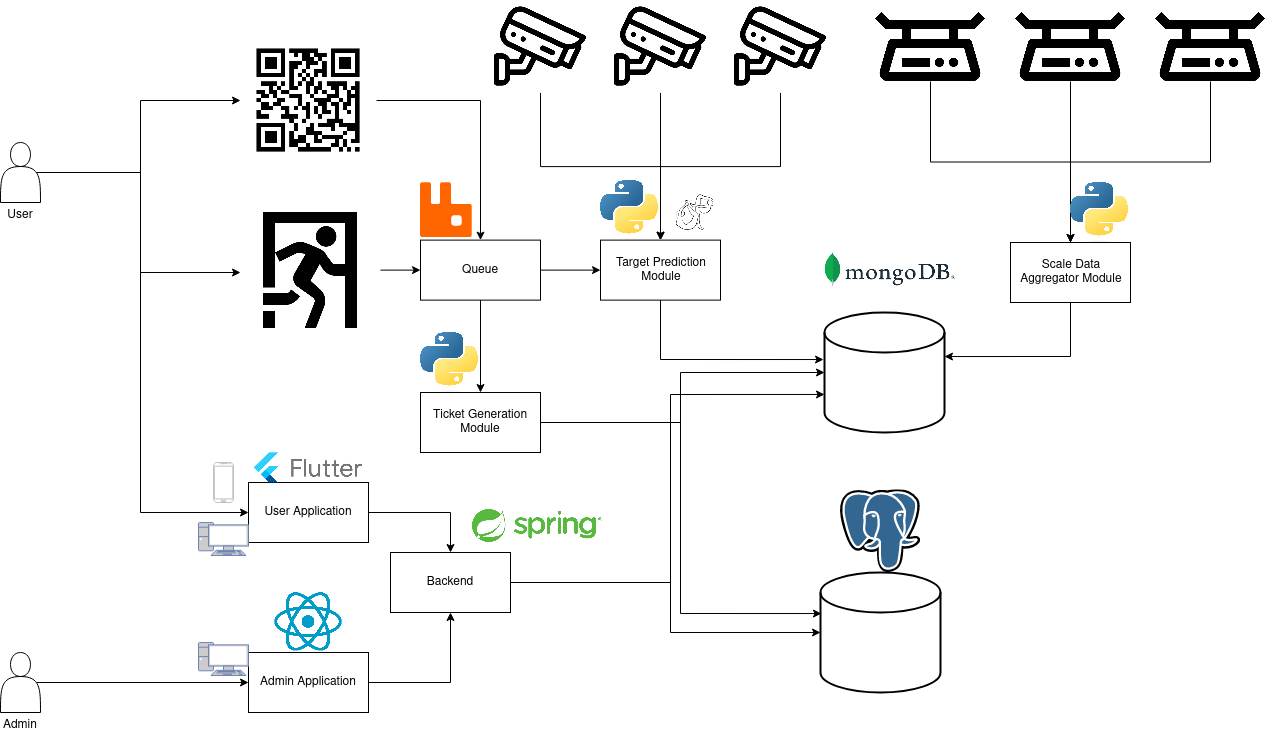
\includegraphics[width=1.05\textwidth]{./Figuras/Arquitectura TDG-Arch proposal.drawio.png}
\caption{Diagrama de arquitectura a alto nivel de como funcionaría el sistema de AiFi.}
\label{fig:arqAifi}
\end{figure}

El sistema está basado en eventos y en información tabular de los productos, su precio, etc. Cuando un cliente termina su compra, el módulo de \textit{Ticket Generation} accede a la información asociada con ese cliente y genera el ticket correspondiente. 

El equipo ganador de la competencia logró un F1 Score de 97,6\%, lo que representa un muy buen desempeño. Sin embargo, se identificó que el sistema no resuelve de manera adecuada los casos extremos, donde se presentan escenarios con varios clientes simultáneos, clientes que mueven productos entre estantes o incluso clientes que dejan los productos fuera de los lugares designados. Estos casos extremos son relevantes, ya que en el uso diario de estos sistemas es más probable que los clientes actúen de manera impredecible o poco ordenada, en contraste con los casos ideales en los que el sistema funciona correctamente.

El enfoque del equipo ganador se centró principalmente en el análisis estadístico de los datos de las balanzas en los estantes, pasando por alto el potencial de las técnicas de visión por computadora para mejorar la capacidad del sistema en los casos extremos.

El desafío concreto en el uso de cámaras es que los productos de venta minorista representan problemas para las arquitecturas más populares de visión por computadora, como por ejemplo:
\begin{itemize}
	\item Una gran dificultad a la hora de diferenciar la versión grande o la versión chica de un mismo producto, pudiendo representar pérdidas
	\item Un fino trabajo de mantenimiento del sistema a la hora de actualizar los productos disponibles
	\item El tiempo requerido para el reentrenamiento es un aspecto crítico, ya que puede depender del acceso a hardware costoso. Además, el proceso de validación y reentrenamiento puede ser prolongado, lo que puede generar desconfianza por parte del dueño del local.
\end{itemize}
Estos son algunos de los problemas no triviales que se deberán contemplar para que la mejora sea efectiva.

El objetivo de este trabajo es mejorar la capacidad del sistema de checkout autónomo desarrollado por el equipo ganador de la competencia. La idea es poder optimizar y perfeccionar la única solución abierta disponible para abordar este problema. Además, se busca realizar una investigación sobre el tema, explorando nuevas perspectivas y enfoques.

\section{2. Identificación y análisis de los interesados}
\label{sec:interesados}


\begin{table}[ht]
%\caption{Identificación de los interesados}
%\label{tab:interesados}
\begin{tabularx}{\linewidth}{@{}|l|X|X|l|@{}}
\hline
\rowcolor[HTML]{C0C0C0} 
Rol           & Nombre y Apellido & Organización 	& Puesto 	\\ \hline
%Impulsor      &                   &              	&        	\\ \hline
Responsable   & \authorname       & FIUBA        	& Alumno 	\\ \hline
%Colaboradores &                   &              	&        	\\ \hline
Orientador    & \supname	      & \pertesupname 	& Director Trabajo final \\ \hline
Cliente    & Locales minoristas que buscan incorporar checkout autónomo	      & - 	& - \\ \hline
Usuario final   & Equipo de mantenimiento y desarrollo de locales que buscan incorporar checkout autónomo       & -        	& - 	\\ \hline
%Equipo        & miembro1 \newline 
				%miembro2          &              	&        	\\ \hline
%Opositores    &                   &              	&        	\\ \hline
%Usuario final &                   &              	&        	\\ \hline
\end{tabularx}
\end{table}

\begin{itemize}

\item \textbf{Cliente}: contempla todos los locales interesados en incorporar la tecnologia de checkout autonomo para mejorar sus procesos.
\item \textbf{Usuario final}: en el equipo de desarrollo y mantenimiento técnico, se incluyen tanto los desarrolladores como los encargados de \textit{devops}. Estos profesionales requerirán herramientas y procesos ajustados a las necesidades del negocio para llevar a cabo eficientemente sus tareas.
\end{itemize}


\section{3. Propósito del proyecto}
\label{sec:proposito}

El propósito de este proyecto es contribuir al avance del conocimiento en el uso de cámaras en sistemas de checkout autónomo, con el objetivo de mejorar la única aproximación de código abierto disponible. En simultáneo, se busca profundizar sobre las diferentes técnicas de visión de computadora y explorar cómo utilizarlas y combinarlas de manera efectiva para desarrollar un predictor adecuado para este problema específico.

\section{4. Alcance del proyecto}
\label{sec:alcance}

El presente proyecto incluye:
\begin{itemize}

\item Actualización y refactorización del código ya existente para mejorar su ergonomía y usabilidad.
\item una investigación sobre las técnicas disponibles y sobre cómo utilizarlas y combinarlas para lograr un predictor adecuado para este problema.
\item Una actualización pertinente de la documentación, para que sea fácil usar y expandir el proyecto, de forma que otros puedan construir sobre este.
\item Implementación de un predictor basado en los imágenes de video del dataset para resolver el problema presentado.
\end{itemize}

El presente proyecto no incluye:
\begin{itemize}
\item Una implementación concreta con la infraestructura que pueda usarse con el software desarrollado.
\end{itemize}


\section{5. Supuestos del proyecto}
\label{sec:supuestos}

Para el desarrollo del presente proyecto se supone que:

\begin{itemize}
	\item El dataset (videos y datos de los sensores) sigue completamente disponible.
	\item El proyecto ganador sigue disponible en GitHub.
	\item Los videos disponibles deben tener un formato procesable.
	\item Debe existir un dataset que contenga imágenes de los productos que se observan en los videos para poder entrenar predictores.
	\item El dataset debe ser consistente, evitando la falta de relación entre los datos de sensores y las observaciones en los videos, garantizando que no haya inconsistencias.
\end{itemize}


\section{6. Requerimientos}
\label{sec:requerimientos}

\begin{enumerate}
	\item Requerimientos funcionales.
		\begin{enumerate}
			\item El sistema debe ser capaz de procesar videos de compras en tiempo real y extraer información relevante de las imágenes, incluyendo la detección de productos. En este contexto tiempo real contempla una demora de hasta 5 minutos luego de finalizada la compra.
			\item El sistema debe utilizar técnicas de visión por computadora para identificar con precisión los productos presentes en el video, incluso en casos de escenarios complejos con varios clientes, movimientos de productos entre estantes y productos fuera de los lugares designados.
			\item El sistema debe ser capaz de distinguir entre diferentes versiones de un mismo producto, evitando confusiones y garantizando una identificación precisa.
			\item El sistema debe mantener actualizado el inventario de productos a medida que se realizan las compras, registrando las cantidades vendidas y actualizando los niveles de stock en tiempo real.
			\item El sistema debe generar un ticket de compra detallado y preciso, incluyendo los productos adquiridos, sus precios y el total a pagar por el cliente.
			\item El sistema debe ser escalable y flexible, permitiendo la incorporación de nuevos productos
		\end{enumerate}
	\item Requerimientos no funcionales.
		\begin{enumerate}
		\item El sistema debe permitir la integración de nuevos modelos de forma sencilla.
			\item El sistema debe ser fácil de mantener y actualizar, con una estructura de código limpia y modular que facilite la incorporación de mejoras y la corrección de errores.
			\item El sistema debe ser robusto y capaz de manejar diferentes tipos de productos, envases y etiquetas.
		\end{enumerate}
		\item Requerimientos de documentación.
		\begin{enumerate}
			\item Se debe proporcionar un informe técnico que describa la arquitectura del sistema, incluyendo diagramas y explicaciones detalladas de los componentes, módulos y su interacción.
			\item El proyecto debe contar con una documentación clara y detallada del código fuente, incluyendo comentarios, explicaciones de las funciones y métodos utilizados, y guías de uso de las diferentes partes del sistema
			\item Se deben documentar las técnicas de visión por computadora utilizadas, incluyendo algoritmos, metodologías y herramientas específicas empleadas en el procesamiento de imágenes y la identificación de productos.
			\item Se debe documentar el proceso de entrenamiento del modelo de visión por computadora, detallando el conjunto de datos utilizado, la preparación de los datos, los algoritmos de aprendizaje automático empleados y los resultados obtenidos.
		\end{enumerate}
\end{enumerate}

\section{7. Historias de usuarios (\textit{Product backlog})}
\label{sec:backlog}

Para la estimación de \textit{story points} se utilizara el siguiente esquema, basado en la complejidad y la dificultad de cada historia de usuario.

\begin{table}[ht]
\centering
\caption{Tabla de Complejidad y Dificultad}
\label{tab:tabla}
\begin{tabular}{|c|c|}
\hline
\multicolumn{2}{|c|}{\textbf{Complejidad}} \\ \hline
\textbf{Baja}   & 1                     \\ \hline
\textbf{Media} & 3                     \\ \hline
\textbf{Alta}  & 8                     \\ \hline
\end{tabular}
\quad
\begin{tabular}{|c|c|}
\hline
\multicolumn{2}{|c|}{\textbf{Dificultad}} \\ \hline
\textbf{Baja}   & 1                      \\ \hline
\textbf{Media} & 2                      \\ \hline
\textbf{Alta}  & 5                      \\ \hline
\end{tabular}
\end{table}

En función a la estimación de complejidad y dificultad se calculará el promedio. Luego se redondeará hacia arriba para conseguir el valor de Fibonacci correspondiente. Este valor será el que corresponda a los \textit{story points} de la \textit{user story}.

\begin{table}[ht]
\centering
\caption{Tabla de asignación de Story Points}
\label{tab:story-points}
\begin{tabular}{|c|c|c|c|}
\hline
\textbf{Complejidad} & \textbf{Dificultad} & \textbf{Promedio} & \textbf{Story Points} \\ \hline
1                    & 1                   & 1                     & 1                 \\ \hline
1                    & 2                   & 1,5                   & 2                 \\ \hline
1                    & 5                   & 3                     & 3                 \\ \hline
3                    & 1                   & 2                     & 2                 \\ \hline
3                    & 2                   & 2,5                   & 3                 \\ \hline
3                    & 5                   & 4                     & 5                 \\ \hline
8                    & 1                   & 4,5                   & 5                 \\ \hline
8                    & 2                   & 5                     & 5                 \\ \hline
8                    & 5                   & 6,5                   & 8                 \\ \hline
\end{tabular}
\end{table}

\begin{itemize}
	\item Como encargado del local, quiero que el sistema genere predicciones con muy alta precisión para mantener el stock actualizado y generar los cobros pertinentes.
	\begin{itemize}
	\item Complejidad: 1.
	\item Dificultad: 5.
	\item Story Points: 3.
	\end{itemize}
	\item Como usuario, quiero que el sistema genere un ticket de compra detallado y preciso, incluyendo los productos adquiridos, sus precios y el total a pagar, para facilitar y garantizar un correcto proceso de cobro.
	\begin{itemize}
	\item Complejidad: 3.
	\item Dificultad: 5.
	\item Story Points: 5.
	\end{itemize}
	\item Como encargado de mantener el sistema, quiero que el sistema sea fácil de mantener y actualizar, con una estructura de código modular y documentación clara, para facilitar las futuras mejoras y correcciones.
	\begin{itemize}
	\item Complejidad: 3.
	\item Dificultad: 2.
	\item Story Points: 3.
	\end{itemize}
	\item Como encargado de mantener el sistema, quiero que el sistema sea escalable y flexible, permitiendo la incorporación de nuevos productos y la adaptación a diferentes configuraciones de cámaras y entornos de tienda, para que pueda crecer y adaptarse a mis necesidades cambiantes.
	\begin{itemize}
	\item Complejidad: 3.
	\item Dificultad: 5.
	\item Story Points: 5.
	\end{itemize}
\end{itemize}

\section{8. Entregables principales del proyecto}
\label{sec:entregables}

Los entregables del proyecto son (ejemplo):

\begin{itemize}
	\item Manual de uso.
	\begin{itemize}
	\item Guía de instalación.
	\item Guía de integración.
	\item Diagrama de arquitectura.
	\item Detalles de la entrada y salida del sistema.
	\item Detalles de los modelos utilizados.
	\end{itemize}
	\item Código fuente.
	\begin{itemize}
	\item Código actualizado con la nueva funcionalidad de visión por computadora.
	\item Uno o más modelos de visión por computadora implementados.
	\end{itemize}
	\item Informe final.
\end{itemize}

\section{9. Desglose del trabajo en tareas}
\label{sec:wbs}

\begin{enumerate}
\item Investigación de técnicas de visión por computadora. (150 h)
	\begin{enumerate}
		\item Investigar técnicas disponibles generalmente para la detección de productos. (40 h)
		\item Investigar técnicas utilizadas por empresas de checkout autónomo para la detección de productos. (30 h)
		\item Investigar técnicas que buscan resolver el problemas de deteccion de productos similares. (40 h)
		\item Investigar técnicas que buscan reducir el tiempo de entrenamiento del modelo. (40 h)
	\end{enumerate}
\item Implementar y probar las mejores soluciones. (150 h)
	\begin{enumerate}
	\item Implementar las mejores 3 soluciones. (75 h)
		\begin{enumerate}
			\item Implementar la mejor solución. (25 h)
			\item Implementar la segunda mejor solución. (25 h)
			\item Implementar la tercera mejor solución. (25 h)
		\end{enumerate}
	\item Realizar pruebas de las soluciones implementadas. (75 h)
		\begin{enumerate}
			\item Realizar pruebas de la mejor solución. (25 h)
			\item Realizar pruebas de la segunda mejor solución. (25 h)
			\item Realizar pruebas de la tercera mejor solución. (25 h)
		\end{enumerate}
	\end{enumerate}
\item Refactorización y limpieza del código. (140 h)
		\begin{enumerate}
			\item Reconocer la estructura del código. (40 h).
			\item Refactorizarlo de forma de mejorar la claridad y ergonomía. (40 h)
			\item Implementar una interfaz para poder desarrollar varios modelos predictores de productos que formen parte del nuevo proceso. (30 h)
			\item Integrar los predictores al código refactorizado. (30 h)
		\end{enumerate}
\item Documentación e informe final. (160 h)
\begin{enumerate}
	\item Inicio elaboración memoria técnica - Taller de Trabajo Final A. (100 h)
		\begin{enumerate}
			\item Desarrollar un reporte de las técnicas investigadas y definir al menos tres soluciones a probar e implementar. (20 h)
			\item Desarrollar un informe de las pruebas realizadas. (20 h)
			\item Documentación del código. (20 h)
			\item Elaboración manuales de uso y reparación. (40 h)
		\end{enumerate}
	\item Revisión y correcciones de la memoria. (5 h)
	\item Fin de elaboración memoria técnica - Taller de Trabajo Final B. (40 h)
	\item Revisión y correcciones de la memoria. (5 h)
	\item Elaboración presentación final. (8 h)
	\item Revisión y correcciones de la presentación final. (2 h)
	\end{enumerate}
\end{enumerate}

Cantidad total de horas: 600 h

\section{10. Diagrama de Activity On Node}
\label{sec:AoN}


\begin{figure}[htpb]
\centering 
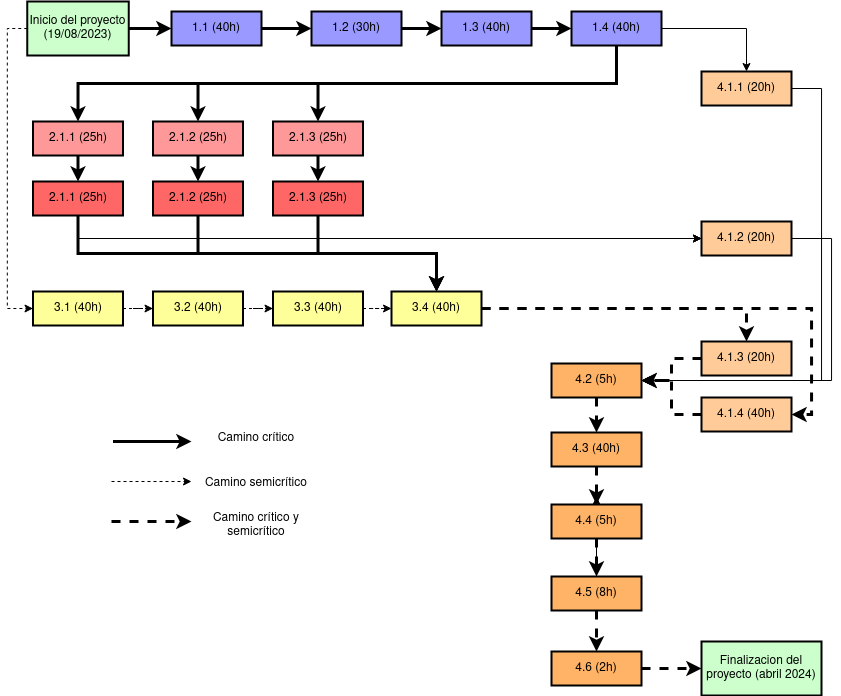
\includegraphics[width=.8\textwidth]{./aon.drawio.png}
\caption{Diagrama de \textit{Activity on Node}.}
\label{fig:AoN}
\end{figure}

En la figura \ref{fig:AoN}, se observa el Activity on Node del proyecto. Caben destacar las siguientes referencias y aclaraciones:
\begin{itemize}
\item Cada nodo contiene una referencia a una tarea del WBS presentado en el punto anterior.
\item Cada grupo de tareas fue agrupado por colores: lila para el trabajo de implementación, rojo para el trabajo relacionado a implementación y prueba de modelos, amarillo para el trabajo relacionado a la refactorización del código y naranja para el trabajo de documentación.
\item Se detallan los caminos crítico y semicrítico, con su referencia correspondiente en la figura.
\item El camino crítico del proyecto es de 360 horas. Es decir, que no podría terminarse antes de las 360 horas de trabajo.
\end{itemize}

\begin{landscape}
\section{11. Diagrama de Gantt}
\label{sec:gantt}
\begin{figure}[htpb]
\centering 
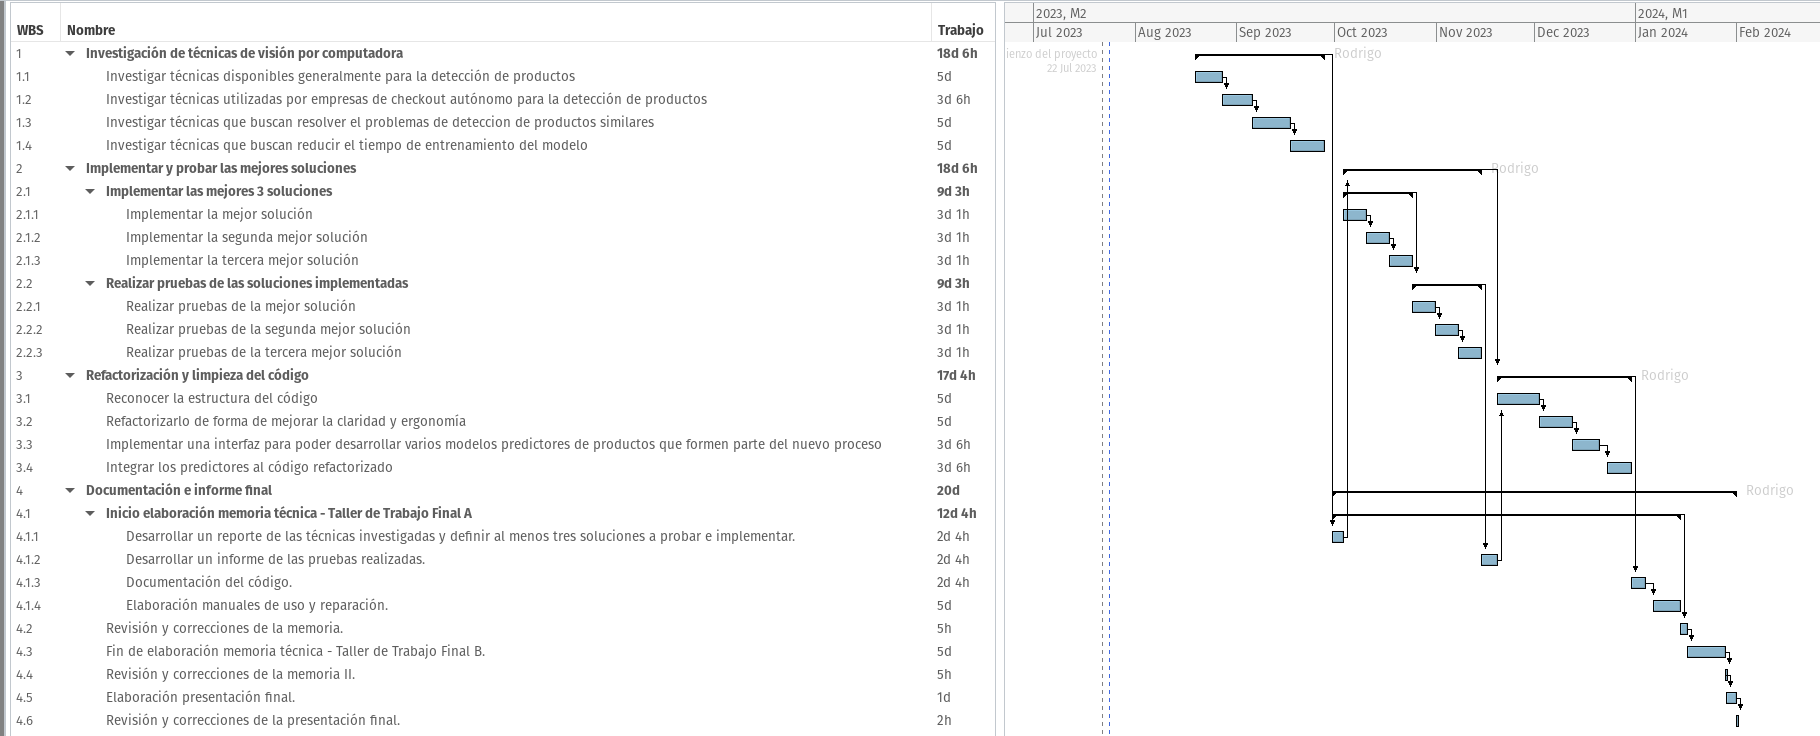
\includegraphics[height=.63\textheight]{./gantt full.png}
\caption{Diagrama de Gantt del proyecto}
\label{fig:diagGantt}
\end{figure}
El diagrama de Gantt que se muestra en la figura \ref{fig:diagGantt} contempla 31 horas de trabajo semanal.
\end{landscape}

\section{12. Presupuesto detallado del proyecto}
\label{sec:presupuesto}

La moneda utilizada para este presupuesto es el peso argentino.

\begin{table}[htpb]
\centering
\begin{tabularx}{\linewidth}{@{}|X|c|r|r|@{}}
\hline
\rowcolor[HTML]{C0C0C0} 
\multicolumn{4}{|c|}{\cellcolor[HTML]{C0C0C0}COSTOS DIRECTOS} \\ \hline
\rowcolor[HTML]{C0C0C0} 
Descripción &
  \multicolumn{1}{c|}{\cellcolor[HTML]{C0C0C0}Cantidad} &
  \multicolumn{1}{c|}{\cellcolor[HTML]{C0C0C0}Valor unitario} &
  \multicolumn{1}{c|}{\cellcolor[HTML]{C0C0C0}Valor total} \\ \hline
 Horas de ingeniería & 
  \multicolumn{1}{c|}{600 h} &
  \multicolumn{1}{c|}{\$ 5.000 / h } &
  \multicolumn{1}{c|}{\$ 3.000.000} \\ \hline
 Alquiler PC Laptop & 
  \multicolumn{1}{c|}{600 h} &
  \multicolumn{1}{c|}{\$ 530 / h } &
  \multicolumn{1}{c|}{\$ 318.000} \\ \hline
 Alquiler PC con placa de video dedicada & 
  \multicolumn{1}{c|}{600 h} &
  \multicolumn{1}{c|}{\$ 1060 / h } &
  \multicolumn{1}{c|}{\$ 636.000} \\ \hline
\multicolumn{1}{|l|}{} &
   &
   &
   \\ \hline
\multicolumn{1}{|l|}{} &
   &
   &
   \\ \hline
\multicolumn{3}{|c|}{SUBTOTAL} &
  \multicolumn{1}{c|}{\$3.954.000} \\ \hline
\rowcolor[HTML]{C0C0C0} 
\multicolumn{4}{|c|}{\cellcolor[HTML]{C0C0C0}COSTOS INDIRECTOS} \\ \hline
\rowcolor[HTML]{C0C0C0} 
Descripción &
  \multicolumn{1}{c|}{\cellcolor[HTML]{C0C0C0}Cantidad} &
  \multicolumn{1}{c|}{\cellcolor[HTML]{C0C0C0}Valor unitario} &
  \multicolumn{1}{c|}{\cellcolor[HTML]{C0C0C0}Valor total} \\ \hline
Espacio de coworking (individual) & 
  \multicolumn{1}{c|}{6 meses} &
  \multicolumn{1}{c|}{\$ 20.000 / mes } &
  \multicolumn{1}{c|}{\$ 120.000} \\ \hline
\multicolumn{1}{|l|}{} &
   &
   &
   \\ \hline
\multicolumn{1}{|l|}{} &
   &
   &
   \\ \hline
\multicolumn{3}{|c|}{SUBTOTAL} &
  \multicolumn{1}{c|}{\$ 120.000} \\ \hline
\rowcolor[HTML]{C0C0C0}
\multicolumn{3}{|c|}{TOTAL} &
   \multicolumn{1}{c|}{\$ 4.074.000} \\ \hline
\end{tabularx}%
\end{table}


\section{13. Gestión de riesgos}
\label{sec:riesgos}

A continuación se listan los riesgos identificados:

\begin{itemize}
\item Riesgo 1: que deje de estar disponible el dataset proporcionado por AiFi.
\begin{itemize}
\item Severidad (10): no se podría llevar adelante la parte más importante del trabajo. La solución sería cambiar de proyecto totalmente.
\item Probabilidad (5): el dataset sigue disponible luego de 3 años. Puede ocurrir que sin previo aviso lo eliminen, pero al día de hoy no sucedió.
\end{itemize}
\item Riesgo 2: que los tiempos de entrenamiento de modelos sean demasiado largos.
\begin{itemize}
\item Severidad (7): los modelos de visión por computadora suelen requerir mucho tiempo de entrenamiento. Este tiempo fue contemplado en la estimación pero puede que esa estimación no se ajuste a la realidad.
\item Probabilidad (4): teniendo una PC con placa de video dedicada (GTX 1660 Super) la probabilidad de que esto ocurra es relativamente baja, considerando el tamaño del dataset con el que se va a trabajar.
\end{itemize}
\item Riesgo 3: que el dataset de productos disponibles no sea útil para el entrenamiento de modelos.
\begin{itemize}
\item Severidad (6): algunos modelos modernos necesitan mucha información para poder lograr soluciones efectivas. Si el dataset no es lo suficientemente grande, estos modelos no serían útiles.
\item Probabilidad (3): existe un abanico de modelos lo suficientemente amplio como para que no todos las soluciones elegidas necesiten un dataset grande.
\end{itemize}
\item Riesgo 4: no encontrar información sobre los modelos/arquitecturas que usan las empresas de checkout autónomo hoy en día.
\begin{itemize}
\item Severidad (2): implicaría no contar con información valiosa, aunque no esencial, de empresas especializadas para seleccionar los soluciones a implementar. 
\item Probabilidad (7): el activo más importante de estas empresas es esta información, por lo que no es algo que suelen compartir. Al mismo tiempo, muchas de estas empresas comparten sus investigaciones y avances para que su solución sea estándar y lograr ser líderes del mercado.
\end{itemize}
\item Riesgo 5: que el trabajo de refactorización sea demasiado extenso para lograr los objetivos de modularización y extensibilidad.
\begin{itemize}
\item Severidad (7): implicaría sumar horas dedicadas al grupo de refactorización. En el peor de los casos, serían 40 horas más de trabajo total.
\item Probabilidad (2): el tiempo asignado a la refactorización se basó en la evaluación del responsable del equipo, que es ingeniero informático. Su evaluación sobre la calidad del código y el trabajo necesario para refactorizarlo tiene pocas posibilidades de no ser representativo.
\end{itemize}
\end{itemize}

En base a lo desarrollado, se construye la tabla de gestión de riesgos. Se calcula el RPN como
la multiplicación de la severidad y la probabilidad de ocurrencia.

\begin{table}[htpb]
\centering
\begin{tabularx}{\linewidth}{@{}|X|c|c|c|c|c|c|@{}}
\hline
\rowcolor[HTML]{C0C0C0} 
Riesgo & S & O & RPN & S* & O* & RPN* \\ \hline
   1   &  10 & 5  &  50   &  1  &  5  &  5    \\ \hline
   2   &  7 & 4  &   28  &  3  &  4  &   12   \\ \hline
   3   &  6 & 3  &   18  &  2  &   4 &   8   \\ \hline
   4   &  2 & 7 &   14 &    &    &      \\ \hline
   5   &  7 & 2  &  14   &    &    &      \\ \hline
\end{tabularx}%
\end{table}

Nota: los valores marcados con (*) en la tabla corresponden luego de haber aplicado la mitigación.

Criterio adoptado: 
Se tomarán medidas de mitigación en los riesgos cuyos números de RPN sean mayores a 15.

\begin{itemize}
\item Riesgo 1: desarrollar un \textit{backup} del dataset. Esta tarea no representa mucho tiempo y esfuerzo.
\begin{itemize}
\item Severidad (1): teniendo el \textit{backup}, representa una severidad baja que el dataset deje de estar disponible en línea.
\item Probabilidad (5): la probabilidad no cambia. 
\end{itemize}}
\item Riesgo 2: por cada uno de los modelos recomendados, desarrollar una lista de al menos dos modelos similares que requieran menos tiempo de entrenamiento.
\begin{itemize}
\item Severidad (3): con una lista de opciones es más fácil cambiar el trabajo sin perder tiempo y sin comprometer la aproximación original al problema. 
\item Probabilidad (4): la probabilidad no cambia. 
\end{itemize}
\item Riesgo 3: si fuera necesario y dentro de lo disponible, extender el dataset con imágenes e información disponible en internet.
\begin{itemize}
\item Severidad (2): con la opción de extender el dataset si fuera necesario, el impacto del riesgo es mucho menor.
\item Probabilidad (4): la probabilidad no cambia. 
\end{itemize}
\end{itemize}

\section{14. Gestión de la calidad}
\label{sec:calidad}

\begin{enumerate}
\item Requerimientos funcionales.
\begin{enumerate}
\item El sistema debe ser capaz de procesar videos de compras en tiempo real y extraer información relevante de las imágenes, incluyendo la detección de productos. En este contexto tiempo real contempla una demora de hasta 5 minutos luego de finalizada la compra.
			\begin{itemize}
	\item Verificación: realizar pruebas de verificación con el dataset original como entrada del sistema.
	\item Validación: realizar pruebas controladas con el cliente en su local.   
\end{itemize}
			\item El sistema debe utilizar técnicas de visión por computadora para identificar con precisión los productos presentes en el video, incluso en casos de escenarios complejos con varios clientes, movimientos de productos entre estantes y productos fuera de los lugares designados.
			\begin{itemize}
		\item Verificación: realizar pruebas de verificación con el dataset original como entrada del sistema, particularmente con los escenarios con varios clientes, movimientos de productos entre estantes y productos fuera de los lugares designados.
	\item Validación: realizar pruebas no controladas con el cliente en su local, con compradores reales.
\end{itemize}
			\item El sistema debe ser capaz de distinguir entre diferentes versiones de un mismo producto, evitando confusiones y garantizando una identificación precisa.
			\begin{itemize}
	\item Verificación: realizar pruebas manualmente con todos los productos que el sistema debería poder identificar.
	\item Validación: realizar pruebas manualmente con todos los productos que el cliente necesita poder identificar.
\end{itemize}
			\item El sistema debe mantener actualizado el inventario de productos a medida que se realizan las compras, registrando las cantidades vendidas y actualizando los niveles de stock en tiempo real.
			\begin{itemize}
	\item Verificación: realizar pruebas de verificación con el dataset original como entrada del sistema.  
	\item Validación: realizar pruebas controladas con el cliente en su local.  
\end{itemize}
			\item El sistema debe generar un ticket de compra detallado y preciso, incluyendo los productos adquiridos, sus precios y el total a pagar por el cliente.
			\begin{itemize}
	\item Verificación: realizar pruebas de verificación con el dataset original como entrada del sistema.  
	\item Validación: realizar pruebas controladas con el cliente en su local.  
\end{itemize}
			\item El sistema debe ser escalable y flexible, permitiendo la incorporación de nuevos productos
			\begin{itemize}
	\item Verificación: una vez terminadas las primeras pruebas manuales de verificación, repetir las mismas pruebas con nuevos productos y el modelo actualizado para soportarlos.
	\item Validación: una vez terminadas las primeras pruebas manuales de validación, repetir las mismas pruebas con nuevos productos y el modelo actualizado para soportarlos.  
\end{itemize}
\end{enumerate}
\item Requerimientos no funcionales.
\begin{enumerate}
\item El sistema debe permitir la integración de nuevos modelos de forma sencilla.
		\begin{itemize}
	\item Verificación: con la documentación necesaria para este proceso, conseguir voluntarios con perfiles similares a los encargados de mantenimiento del sistema y pedirles que sigan las instrucciones y evalúen su efectividad. 
	\item Validación: con la documentación necesaria para este proceso, pedirles a las personas encargadas del mantenimiento que sigan las instrucciones y evalúen su efectividad.
\end{itemize}
			\item El sistema debe ser robusto y capaz de manejar diferentes tipos de productos, envases y etiquetas.	
			\begin{itemize}
		\item Verificación: una vez terminadas las primeras pruebas manuales de verificación, repetir las mismas pruebas con productos idénticos pero con diferentes envases y etiquetas.
	\item Validación: una vez terminadas las primeras pruebas manuales de validación, repetir las mismas pruebas con productos idénticos pero con diferentes envases y etiquetas. 
\end{itemize}	
\end{enumerate}
\item Requerimientos de documentación.
\begin{enumerate}
\item Se debe proporcionar un informe técnico que describa la arquitectura del sistema, incluyendo diagramas y explicaciones detalladas de los componentes, módulos y su interacción.
			\begin{itemize}
	\item Verificación: conseguir voluntarios con perfiles similares a los encargados de mantenimiento del sistema, pedirles que lean la documentación y que den una devolución sobre la misma, en función a su claridad y utilidad.
	\item Validación: pedirles a los encargados de mantenimiento del sistema que lean la documentación y pedirles una devolución sobre la misma, en función a su claridad y utilidad.
\end{itemize}
			\item Se debe documentar el proceso de entrenamiento del modelo de visión por computadora, detallando el conjunto de datos utilizado, la preparación de los datos, los algoritmos de aprendizaje automático empleados y los resultados obtenidos.
			\begin{itemize}
	\item Verificación: conseguir voluntarios con perfiles similares a los encargados de mantenimiento del sistema, pedirles que lean la documentación y que den una devolución sobre la misma, en función a su claridad y utilidad.
	\item Validación: pedirles a los encargados de mantenimiento del sistema que lean la documentación y pedirles una devolución sobre la misma, en función a su claridad y utilidad.
\end{itemize}
\end{enumerate}
\end{enumerate}

\section{15. Procesos de cierre}    
\label{sec:cierre}

\begin{itemize}
\item Análisis de cumplimiento del plan de proyecto.
\begin{itemize}
\item Responsable: Rodrigo Pazos.
\item Actividades a realizar: comprobar fecha de finalización real del trabajo respecto
a estimada en la planificación, contrastar horas invertidas en cada tarea, analizar
porcentaje de requerimientos alcanzados correctamente y comprobar si el presupuesto
anticipado fue preciso.
\end{itemize}
\item Análisis de la efectividad de las técnicas utilizadas.
\begin{itemize}
\item Responsable: Rodrigo Pazos.
\item Actividades a realizar: presentar un resumen de las técnicas utilizadas en todos los grupos de trabajo, con sus resultados de calidad, problemas encontrados, soluciones aplicadas, una evaluación de qué tan eficientes fueron y recomendaciones de cómo se podrían conseguir mejores resultados, si fuera necesario. Comparar los riesgos analizados con los problemas encontrados y determinar si alguno de los problemas pudo haber sido considerado dentro de los riesgos del proyecto.
\end{itemize}
\item Acto de agradecimiento.
\begin{itemize}
\item Responsable: Rodrigo Pazos.
\item Actividades a realizar: al finalizar la defensa del trabajo, se agradecerá al director
del proyecto, miembros del jurado, profesores y directivos de la carrera. Se destacarán aportes valiosos del director y profesores. 
\end{itemize}
\end{itemize}


\end{document}
